\begin{quote}
	\textit{``If the chaos of the nineties reflects a radical shift in the paradigms of visual literacy, the final shift away from the Lascaux/Gutenberg tradition of a pre-holographic society, what should we expect from this newer technology, with his promise of discrete encoding and subsequent reconstruction of the full range of sensory perception?''}
\end{quote}
\hfill \textit{Burning Chrome, William Gibson}
\\
\\

%=========================================================================================================

\label{chapter-conclusions}

Alternate realities have fascinated mankind since early prehistory and with the advent of the computer and the smartphone we have seen the rise of many different categories of alternate reality that replace, augment, diminish and mix with our familiar real world to expand our capabilities, our understanding and our entertainment. This thesis has introduced parallel reality as a new category of alternate reality that comprises two environments, one real and the other virtual, each complete unto itself and wherein the user may freely switch between them. The benefits that such a system imparts upon the user by granting them the ability to explore parallel real and virtual environments in tandem has been shown by developing a parallel reality platform, Mirrorshades, and applying it to a use case within the realm of cultural heritage, with evaluation of these studies leading to a number of best practices for future parallel reality endeavours.

\begin{figure}[h]
	\begin{center}
		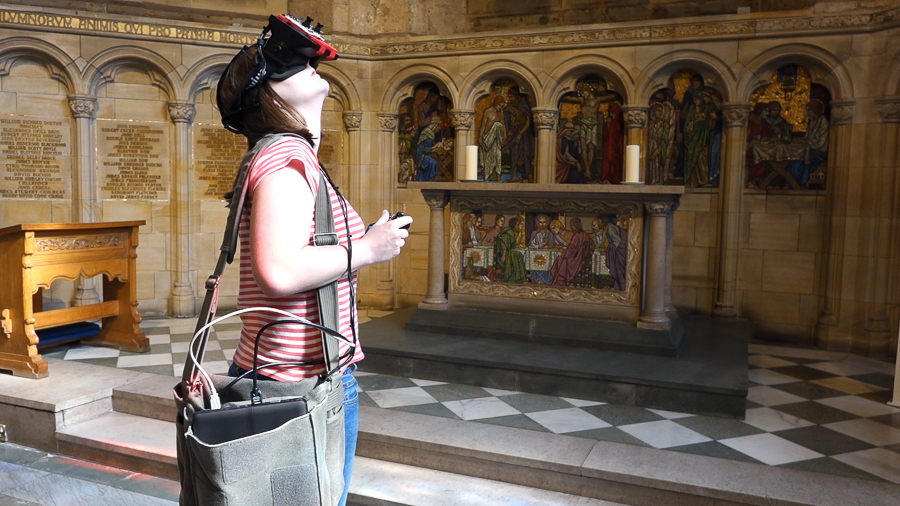
\includegraphics[width=\textwidth]{participant-f-4.jpg}
		\caption{The \textit{Mirrorshades} parallel reality platform in use.}
		\label{participant-f-4.jpg}
	\end{center}	
\end{figure}

%=========================================================================================================

\section{Contributions}

As listed in section \ref{intro-contributions} the contributions of this thesis can be summarized as follows;

\begin{itemize}
	\item The introduction of parallel reality as a new category of alternate reality that allows users to experience two complete environments in tandem and represents an approach for mitigation of the vacancy problem.
	\item The framing of parallel reality through a thorough investigation and extension of previous taxonomies that classify and distinguish alternate reality terminologies.
	\item The creation of the combined Milgram/Waterworth model for visualising alternate reality experiences, including those of parallel reality systems.
	\item Development of a parallel reality platform, dubbed Mirrorshades, that combines new virtual reality hardware with novel indoor positioning technology.
	\item Evaluation of the Mirrorshades platform through user studies of a real world use case study within the realm of cultural heritage, including the application of an established presence questionnaire to parallel reality.
	\item Discussion and creation of a set of best practices for future parallel reality endeavours.
\end{itemize}

%=========================================================================================================

\section{Future Work}

The introduction of parallel reality in this thesis along with the investigation of its first serious implementation in Mirrorshades is only the beginning of en extended course of study that will be required to fully understand and come to appreciate the benefits that the concept can provide. The following highlights a few choice avenues in which the investigation into parallel reality would do well to pursue, but should be no means be considered an exhaustive list of possible improvements and extensions.

Most evident is the matter of hardware. The parallel reality platform presented by this thesis, Mirrorshades, is a somewhat cumbersome package of HMD, laptop, battery pack, smartphone, games console controller and myriad cables, occupying both of the users hands and requiring them to carry a satchel of not insubstantial size and weight. To posit that this cumbersome nature of the platform had a directly detrimental effect upon the quality of experience received by the participants is no stretch of the imagination and improvements in this regard will be required for parallel reality to see deployment and use in anything but controlled laboratory or user study conditions. As discussed in section \ref{mobile-client} we are already beginning to see the advent of hardware platforms that would present a much improved basis for parallel reality experiences. A platform such as Samsung Gear VR, once appropriately modified with the requisite stereo video see-through provision, would represent a fully contained single unit parallel reality experience, suitable for handing to a user in the same manner that audio guides are given out at many of the world's museums. Furthermore, improvements to the performance of the platform, in terms of the visual acuity of both real and virtual content, as well as the accuracy of the positioning and registration, will present beneficial results both to casual users and to experts wishing to use such a modality of interaction for serious study.

Investigating the application of parallel reality to other domains represents possibly one of the largest avenues of potential further extension. While the user studies discussed in this thesis experimentally showed the worth of parallel reality when applied to cultural heritage, parallel reality as a concept can be applied to many fields. Postulating for but a moment, one can imagine how parallel reality could be applied to architecture and visualisation of renovations, using the physical layout of an environment as a canvas for novel artistic expression, to the study of PolySocial interactions involving real and VR parties and new styles of gaming that merge both real and virtual play fields. As society becomes more familiar with and more dependent upon almost constant connection to the virtual, whether in the form of 2D Web based social networks and apps or richer multimedia experiences, the utility of platforms that allow real and virtual environments to be cycled between in a trivial manner will present many exciting applications for parallel reality, including in as yet unforeseen areas.

In addition to other domains, the application of a parallel reality system to more expansive environments should also prove to be a fruitful avenue of investigation. In the evaluation presented in this thesis, participants were restricted to the area inside St Salvator's chapel, however from a conceptual perspective there is nothing to prevent parallel reality from being deployed on larger scales. Allowing a user of a parallel reality system to move between indoor and outdoor areas would require the integration of multiple positioning systems, at least one for indoor areas and a second for outdoor areas, and as the virtual environment grows in tandem with the increasing area of the real world available to the user a switch from static content stored upon the local client to dynamically streamed content will likely be required.

Finally, the experience of using a parallel reality system has been assessed in this thesis only in relation to a traditional seated VR experience within a cultural heritage scenario and from a presence perspective. This represents only a small foray into the sources of study and evaluation that could (and perhaps should) be applied to parallel reality systems, especially when one considers applications in different domains, on larger scales and with the introduction of other users, both real and virtual. Furthermore, all of the evaluation of parallel reality in this thesis has been based upon experiences with a parallel reality system that features high spatial equivalence (see section \ref{spatial-equivalence}) between its real and virtual environments. The application of parallel reality to scenarios that feature little or no spatial equivalence between their environments will surely open up a wealth of exciting investigations.

%=========================================================================================================

\section{Final Thoughts}

While mankind may yet be many decades away from the realisation of a Neil Stephenson-esque metaverse, in which a persistent 3D multi-user virtual environment forms the basis of all of our computer mediated communication and commands as much of our attention as our smartphones do today, the parallel reality concept introduced by this thesis has provided a glimpse of how a novel new category of alternate reality can allow us to interact in tandem with both an immersive 3D environment and the real world around us. While such a platform can already claim some small success in improving the experience of virtual heritage content, the possible applications of such a technology will surely only expand as we continue to integrate more virtuality into our daily lives and come to question our experiences as Orlan proposed (emphasis original);

\begin{quote}
	\textit{``I come back therefore to my initial words about the `\textbf{and}' in order to propose the virtual \textbf{and} the real used simultaneously as new transversalities that question art and the becoming of our world.''}~\cite{Orlan2002}
\end{quote}

%=========================================================================================================